 %% 正文

\chapter{绪论}

\section{研究背景}
大容量、低成本、高性能的存储系统设计一直是存储领域研究的热点,而且随着大数据云存储时代的到来,人们对这样的存储系统的要求更加迫切。而传统的磁盘虽然容量大价格低,但磁盘的机械特性导致了它的性能在很大程度上已经到达极限。因此人们将希望寄托于新型的存储介质上,比如闪存存储器和相变存储器等。近年来固态硬盘已经成为固态硬盘(SSD)已经成为固态技术中的领先技术,最常见的SSD都是基于NAND Flash芯片设计的。SSD以闪存作为存储介质,具有随机读取速度快,功耗低,抗震性好等优点。因此目前广泛运用于家用和企业市场,在发展中的云存储系统中渐渐取代了传统的普通机械硬盘。


但是,目前依然存在一些问题,比如在对数据安全性要求高的场合,普通的SSD组成的阵列无法保证数据的安全。另外,由于SSD固有的特点,被删除的数据依旧可能被非法窃取,导致数据泄露等安全事故。针对这些存在的问题,本研究旨在固态盘阵列存储系统之上设计一套冗余存储方案,存储的数据经过与其哈希信息复杂运算后,生成冗余的加密数据,只要在物理意义上完全删除哈希信息或者一定量的数据块,原始数据即无法恢复,保证数据的安全。


固态盘的特性决定了,普通删除方式是根本不可能“真正”删除数据的,数据依然存在物理介质上\cite{ssd-outofplace-and-trim}。在对闪存页(page)写操作时,需要首先进行块擦除操作,因此,不能对闪存进行就地更新(in-place-update)的操作,只能采用异地更新(out-of-place update)的写方式,这就导致了旧的数据在某个时间窗口内依然存留在闪存上,删除操作只是系统反馈的一个“假的”删除成功。数据删除整个过程如\autoref{fig:1}所示。
\begin{figure}
\centering
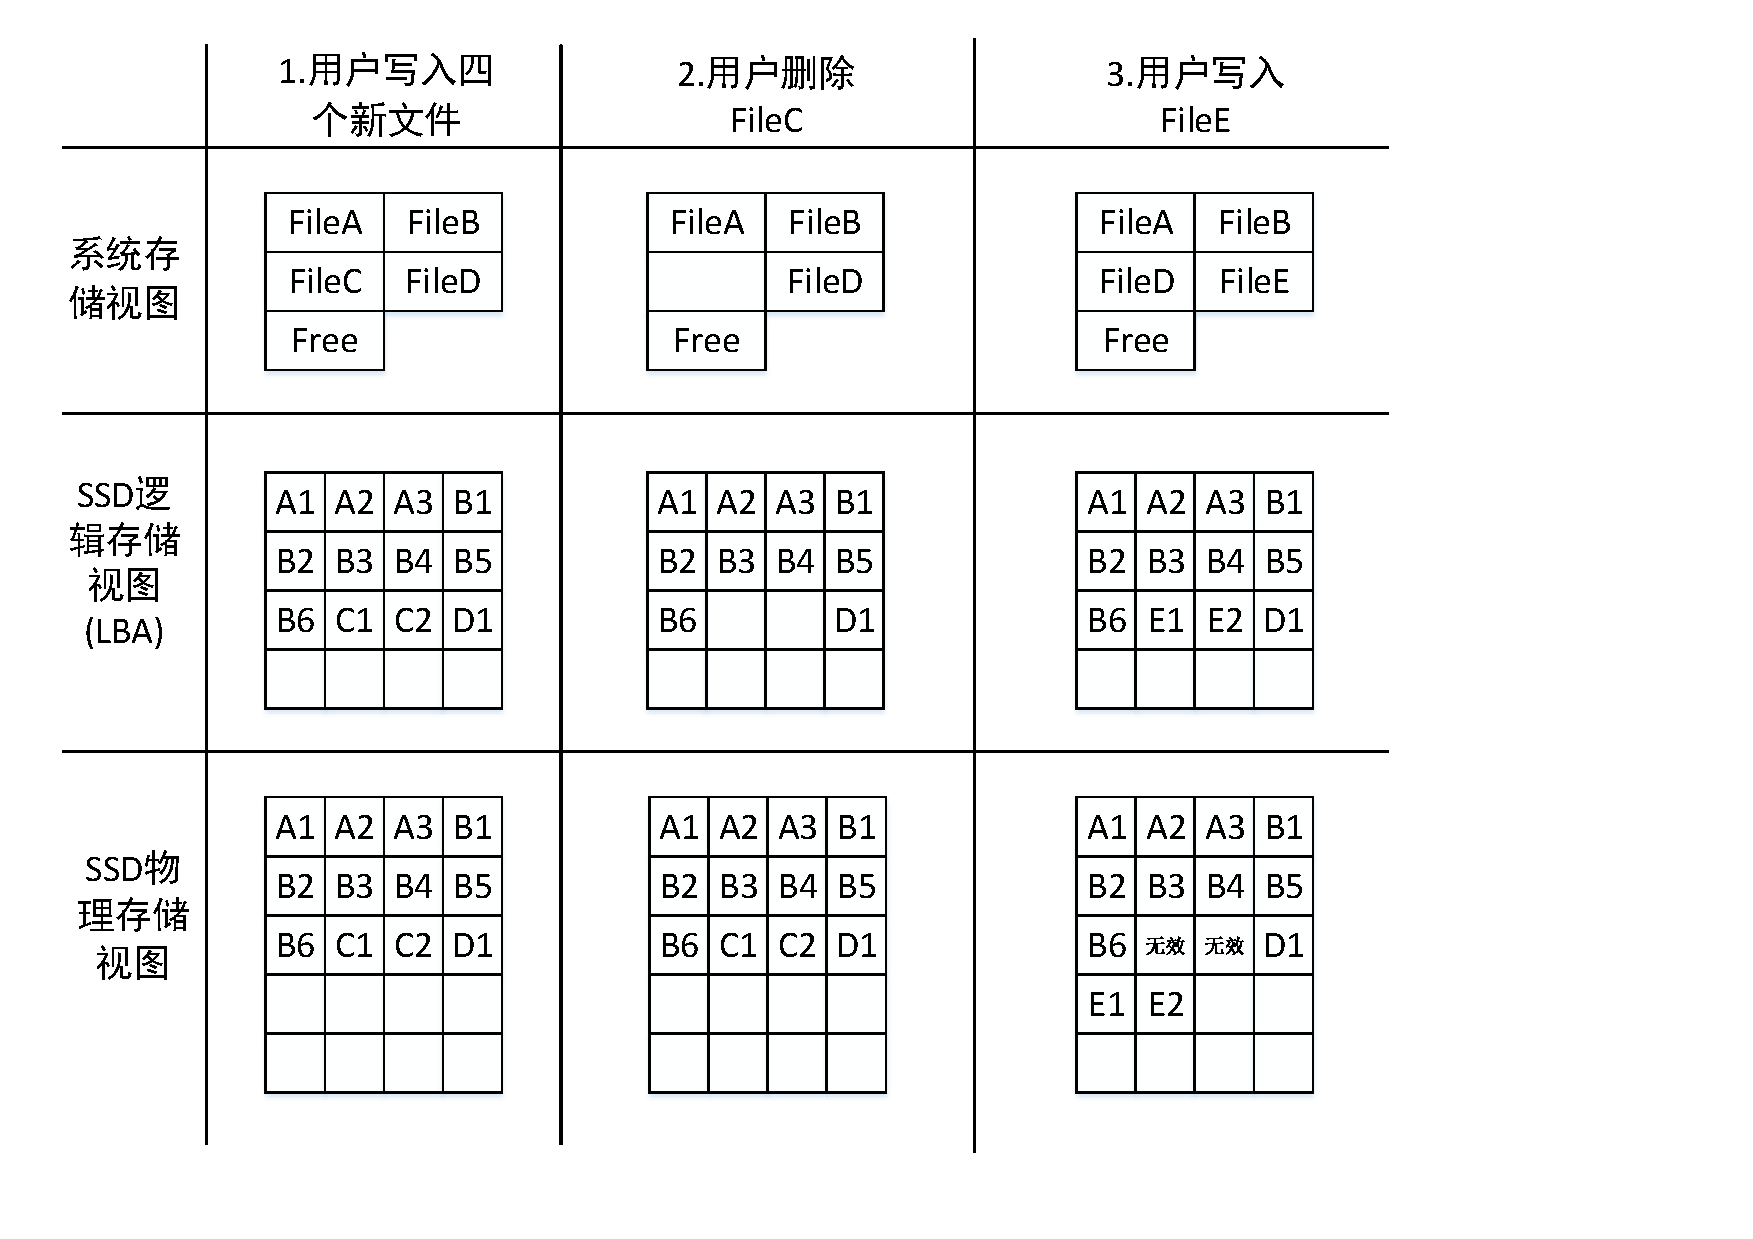
\includegraphics[width=4in]{Pics/fig-out-of-place.pdf}
\caption{固态盘异地更新}\label{fig:1}
\end{figure}
用户在文件系统上首先创建了FileA、FileB、FileC、FileD四个文件数据,反映到固态盘的逻辑块存储视图上的数据,以及在固态盘物理介质上的数据块分别如\autoref{fig:1}所示。
当用户在系统中删除了文件FileC,但是在固态盘的逻辑存储地址和物理介质上,文件C的两个数据块C1、C2却没有删除,也就是说,在用户删除文件数据的时候,数据依然存在。系统只是简单的返回一个“删除成功”的假象给用户。


第三步用户写入新的文件FileE时,虽然在固态盘逻辑块存储地址上,数据块C!,C2的位置被重新写入了新文件FileE的存储地址,但是,在固态盘物理介质上,数据块E1、E2是写入到新的位置,而旧的数据块C1、C2只是被固态盘的垃圾回收标记为“可回收”状态,真正被擦除的时机是不可控的。


从\autoref{fig:1}的三个简单操作可以发现,当用户删除了文件FileC之后,在物理介质上它的数据C1、C2在回收之前,一直都没有真正地被删除掉,这就是固态盘“异地更新”的特性,利用固态盘的这个特性,攻击者使用一些安全工具依然可以将被删掉的文件FileC恢复出来,这就造成了数据被窃取的风险。


怎样设计一套针对全闪存盘阵的安全删除方案,使得用户在物理介质上删除了密钥数据之后,存储的数据就能够保证安全,这就就是我们课题要研究的重点。
\section{研究目的和意义}
在信息化时代,经济、军事领域对于数据的安全性要求是比较高的。由于关键信息的泄露,可能导致国家或者个人非常重大的损失。目前,数据泄露主要存在以下三个问题:


\textbf{(1) 在数据处理、传输、存储等中间过程中,数据可能被非法复制窃取。}
例如网络传输的邮件等可能会被第三方服务商缓存下来,这种不可预知的数据复制操作在互联网时代更加普遍。导致一些企业用户纷纷兴建私有的数据中心,而不是接受公有云的服务,就是为了规避这类问题的风险。


\textbf{(2) 由于不同存储介质的特性不同,导致用户很难真正地删除数据。}虽然针对磁盘已存在很多安全工具,如 O\&O SafeErase、DataWipe、BCwipe、HDDerase、SDelete、Secure Eraser 等\cite{safe-erase,secure-eraser,bcwipe} ,这些工具基本是使用特定数据对目标文件逻辑页多次写入。对于固态盘这样的新型介质, 这些安全删除工具就不起作用。不同介质的存储设备在提供存储服务时,用户很难针对不同的设备使用不同的安全删除手段清除数据,很有可能导致数据泄露。


\textbf{(3) 数据安全删除手段可能降低存储设备或系统的可靠性以及性能。}由于工艺制程的提高,固态盘的线宽发展得更小,每单元存储的数据也越来越多,擦除寿命也变得更短\cite{Yaakobi2012Characterization,Shibata2012A}。\autoref{tab:1}显示了闪存芯片从SLC发展到QLC的线宽、擦除寿命等数据。从表中可以看出,随着闪存芯片的发展,数据安全删除的次数是不断下降的,因此,对于数据安全的删除操作,会减少闪存芯片的剩余擦除次数,使其擦除寿命降低,可能会导致坏块的增多,降低其性能,擦除操作过多更有可能导致不可预期的问题出现,影响存储设备的可靠性。
\begin{table}
\centering
\caption{SLC、MLC、TLC、QLC 四种闪存芯片的特性}\label{tab:1}
    \begin{tabular}{|*{5}{c|}}
\hline
    \multirow{2}{*}{闪存特性} & SLC & MLC & TLC & QLC \\
    & (Single-Level Cell) & (Multi-Level Cell) & (Triple-Level Cell) & (Quad-Level Cell) \\
\hline
    \textbf{存储单元模型} & 每单元一位数据 & 每单元两位数据 & 每单元三位数据 & 每单元四位数据 \\
\hline
    \textbf{速度} & 特别快 & 快 & 慢 & 很慢 \\
\hline
    \multirow{6}{*}{\textbf{擦除寿命}} & 10 万次 & 1万次 & 2500次 & 约500次 \\ %\multirow{2}{*}{约500次} \\
        & (5×nm) & (5×nm) & (5×nm) & \\ \cline{2-5}
    & 10 万次 & 5000次 & 1250次 & N/A \\%\multirow{2}{*}{N/A}  \\
        & (3×nm) & (3×nm) & (3×nm) &\\ \cline{2-5}
    & N/A & 3000次 & 750次 & N/A \\ %\multirow{2}{*}{N/A} \\
        & (2×nm) & (2×nm) & (2×nm) & \\ \hline
\end{tabular}
\end{table}


上述的三个问题说明了,一方面,数据的安全性需要做到安全删除,另一方面,研究基于固态盘阵的数据安全删除是一项有意义的工作,国内外的研究工作都处于起步阶段,积极投身这个领域将会为我国的存储安全研究打开新的局面。

\section{国内外研究现状}
近几年来,针对固态盘的安全删除技术受到了广泛关注。在国内,包括华中科技大学、中南大学、武汉大学等高等院校和科研机构都开展了相关课题和理论的研究。在国外,美国的华盛顿大学、哥伦比亚大学以及IBM、HP等实验室也积极地投身在安全删除领域的研究上。
\subsection{基于密码学意义上的安全删除}
数据在被加密存储之后,如何保证删除密钥数据,原来的数据就无法再被还原,成为新的难题。Perlman等人首次提出了基于时间的数据安全删除方法,针对加密文件,如果密钥过期后数据即被删除,而且文件无法恢复\cite{Perlman2005File}。受Perlman等人的启发,Tang等人设计出了FADE系统\cite{Tang2012Secure},该系统使用公钥密码并使用简单的布尔操作来调整安全删除策略。但是FADE只支持一到两层的布尔表达,而且需要使用复杂的公钥系统。Perlman等人还设计了Ephemerizer系统\cite{Perlman2005The,Tang2009Timed},该系统需要一个可信服务器保存并管理由数据拥有者指定过期时间的解密密钥。Geambasu 等人给出了一个基于时间的数据可信删除方法的原型 Vanish\cite{Geambasu2009Vanish},但Vanish容易受到跳跃攻击(hopping attack)和嗅探攻击(sniffing attack)\cite{Wolchok2010Defeating} 。华中科技大学武汉光电国家实验室曾令仿等人提出了一种SafeVanish\cite{Zeng2010SafeVanish}方案,通过扩展密钥等份长度的方法提高跳跃攻击的成本,并且引入公钥密码体制抵御嗅探攻击,显著改善了Vanish方案。Reimann等人\cite{Reimann2012Timed}针对Vanish系统中当文件在 8 小时后需要被访问时,文件拥有者需要更新节点缓存中的密钥部分问题,提出了将密钥分量分发到随机的网页中保存的改进方案,随着时间的改变,网页会改变存储内容或是被删除。
针对以Vanish为代表的加密方案存在的单个密钥加密全部数据不能对数据进行细粒度的管理等问题,武汉大学王丽娜等人\cite{王丽娜2012一种适于云存储的数据确定性删除方法}提出了利用秘钥生成树,门限秘密共享(threshold secret sharing)来组织和管理秘钥,同时利用分布式散列表(distributed hash table,DHT)周期性地删除相关秘钥来实现安全删除。中南大学王国军等人改进了Vanish方案,除了将密钥分发到 DHT 网络中,还提取部分密文并分发到DHT 网络中,从而更有效抵抗传统密码分析和暴力攻击\cite{Wang2010A}。西安电子科技大学马建峰和中国科学院信息工程研究所李凤华所在课题组针对网络内容生命周期隐私保护问题,提出了面向网络内容隐私的基于
身份加密的安全自毁方案\cite{熊金波2014云计算环境中的组合文档模型及其访问控制方案,熊金波2014基于属性加密的组合文档安全自毁方案,熊金波2014面向网络内容隐私的基于身份加密的安全自毁方案},这种方案基于身份的加密和分布式Hash表(DHT)网络。这些方案更多的是偏向上层应用,在原型系统方面的实现和方法验证方面显得不足。针对密钥从物理介质上“真正地”删除,这些方案涉及的研究都不是很深。
\subsection{物理介质上数据安全删除}
面对这一问题,研究者有的提出了从物理损坏或者化学破坏的方式,这种方法不本方案不涉及相关研究。
M.Wei的一个研究\cite{Wei2011Reliably}表明:
\begin{enumerate}
\item 存储介质的内建命令通常能提供有效的数据擦除功能,但是并不能保证这些命令总是被制造商正确地实现
\item 将SSD的所有数据全部覆盖两次(在大部分情况下)能够有效地清除数据
\item 对于单个数据块删除而言,当前的SSD都存在不足之处
\end{enumerate}


因此,这一过程的实现并不一直是正确的,在有些情况,文件系统显示已被删除,而数据仍在设备中存在。Peterson等人\cite{Peterson2005Secure}在
数据块层使用全有或全无的转换技术(AONT)来实施安全删除,该方法通过AONT存储每一个数据块,然后覆盖其中的一部分,这使得整个数据块不可用。2012年,Diesburg提出TrueErase\cite{Diesburg2012TrueErase},一种类似于TRIM指令的功能,但是只针对属于某敏感文件的数据块。他们在文件系统和设备驱动之间增加了一个新的传输通道。被修改的设备驱动一旦接受到被删除块的信息,使用其下层的接口就可以实现快速安全删除。TrueErase比TRIM更有效,因为它可以只是安全擦除部分敏感块。TrueErase改造了存储管理层,
全方位监控敏感文件的编辑和更新,并可彻底删除敏感文件,前提是假设文件系统可以直接访问和操作物理闪存,所以其缺点是无法应用于普通固态盘。


总体来说,针对全闪存盘阵应用场景,目前研究都处在初始阶段,需要采用新的架构来保证数据的安全删除\cite{傅颖勋2013安全云存储系统与关键技术综述}。现有研究偏向
上层应用,并且越是接近上层系统越抽象,数据确定性删除就越困难\cite{Reardon2013SoK},也难以在存储性能、计算开销和数据通信延迟方面达到很好的平衡\cite{李晖2014公共云存储服务数据安全及隐私保护技术综述}。另外,现有研究缺乏从数据按需删除的角度,只针对敏感数据实施安全删除,从而并不改变普通用户的使用习惯,或根据不同的安全级别需求采取“合理”的数据安全删除策略。
\section{本文的研究内容}
本研究旨在提供一种基于闪存盘组成的阵列的数据安全删除方案。通过对数据进行冗余加密,保障数据安全存储,即高可靠性和高安全性。一方面,采用了非对称加密算法、群域运算保障数据可靠性;另一方面,在编码前引入加密的方式增强数据隐私保护,利用冗余编码的特性结合弱密钥思想,对数据的删除不再需要对整个数据进行覆盖写,而是删除部分数据块,破坏数据完整性或者密钥完整性,使数据无法正常读取。即使攻击者得到数据,也不能获取明文,达到数据安全删除的目的。本研究在保证数据安全存储的同时,降低了对固态盘阵列的读写访问,相当于延长了固态盘的使用寿命。
